\section{The optimal control problem}
\label{sec:ocp}
%\section{The generic optimal control formulation underlying the locomotion problem}

The dynamics \eqref{eq:momentum} corresponds to the difficult part to control on a humanoid robot. It is not directly controllable by the joint torques $\bm \tau_q$ but only indirectly by the contact wrenches $\bm\phi$.
It is also the part of the dynamics that is unstable (because of the cross-product with $\bm c$ on the second line, that will grow exponentially if something goes wrong). On the other hand, if the robot has enough torque (which current high-performance humanoid robots usually have) it will always be possible to find $\bm \tau_q$ to satisfy the actuated part of the dynamics if \eqref{eq:momentum} is satisfied.

Walking pattern generators (WPG) therefore focus on \eqref{eq:momentum} (or on a reformulation of it) to find a valid trajectory of $\bm c$ and $\am$ satisfying the contact constraints $\mathcal{K}$. In this direction, a very classical hypothesis to keep the problem simple is to assume that all the contacts are on a flat ground where slippage is impossible ($\mu = +\infty$), but recent contributions have been proposed to get rid of this hypothesis in a satisfactory manner \cite{kudruss_ichr15,rotella_humanoid15,perrin_isrr15}. In this section, we propose an original formulation of a WPG that is able to handle any distribution of contacts with real-time capabilities.

In a first time, we present an optimal control problem (OCP) under a generic form that represents the problem of computing walking patterns. This form is not suitable for efficient resolution but can be seen as a generic template that covers several previous WPG. We then propose a new formulation that makes an interesting trade off between efficiency and generality. The last part of the section shows how the solution to this problem can be efficiently computed using a particular direct approach.

\subsection{The generic optimal control problem}

We consider the central dynamics \eqref{eq:momentum} along a finite-time trajectory. The state of the problem is composed of the COM position and the momentum. We denote it by $\bm x = (\bm c,\bm h,\am)$. The control of this dynamic system is $\bm u = \bm\phi$ the contact wrench. Eq. \eqref{eq:momentum} can be easily reformulated as 
\begin{equation} \label{eq:dynbilin}
 \dot{\bm x} = f(\bm x,\bm u) = F_x \bm x + F_u(\bm x) \bm u 
\end{equation}
where $F_x$ and $F_u(\bm x)$ are two matrices easily deduced from \eqref{eq:momentum}. We denote by $\underline{\bm x}$ and $\underline{\bm u}$ the state and control trajectories.

Starting with a sequence of contacts, we are interested in computing a feasible trajectory for the under-actuated dynamics, satisfying the Newton-Euler equations, path and terminal constraints. This can be achieved by setting the following OCP over all the sequence:

\begin{subequations} \label{eq:ocpgen}
\begin{eqnarray}
\hspace{-3em}	\underset{\substack{\hspace{2.2em} \underline{\bm x}=(\bm c, \bm h, \am), \\ \underline{\bm u}=\bm\phi} }{\min } \ \ \  
	& & \hspace{-3em} {\sum_{s=1}^S} \int_{t_{s}}^{t_{s}+\Delta t_s\hspace{-4em}} \ell_{s} (\bm x, \bm u) \, dt \label{eq:cost} \\
	s.t. & \forall t & \dot{\bm{x}} = f(\bm x, \bm u) \label{eq:dyn_constraint} \\
	&  \forall t& \bm\phi \in \mathcal{K} 	\label{eq:conic_constraint} \\
        &  \forall t& \am \in \mathcal{B}_\am \label{eq:am_constraint} \\ 
	& & \bm x(0) = \bm x_{0}  \label{eq:init_constraint} \\
	& & \bm x(T) \in \mathcal{X}_* \label{eq:term_constraint}
\end{eqnarray}
\end{subequations}
where $t_{s+1} = t_s+\Delta t_s$ is the start time of the phase $s$ (with $t_{0} = 0$ and $t_{K} = T$). 
Constraints \eqref{eq:dyn_constraint} and \eqref{eq:conic_constraint} enforce a consistent dynamics with respect to the contact model.
Constraint \eqref{eq:am_constraint} imposes some bounds on the angular momentum (or its variation).
Constraint \eqref{eq:init_constraint} imposes the trajectory to start to a given state (typically estimated by the sensor of the real robot).
Constraint \eqref{eq:term_constraint} typically imposes the terminal state to be viable \cite{wieber_humanoid08}.
The cost \eqref{eq:cost} is typically decoupled $\ell_s(\bm x,\bm u) = \ell_x(\bm x) + \ell_u(\bm u)$ whose parameters may vary depending on the phase. $\ell_x$ is generally used to regularize and to smooth the state trajectory while $\ell_u$ tends to minimize the forces, then producing a more dynamic movement. The resulting control is stable as soon as $\ell_x$ comprehends the L-2 norm of one time derivative \mbox{of $\bm c$ \cite{wieber_handbook15}}.

\subsection{Previous formulations}
Problem \eqref{eq:ocpgen} is a difficult problem to solve in its generic form. It seems in particular difficult to find a closed-form of the viable states $\mathcal{X}_*$, or an equivalent form suitable for numerical resolution. 
Similarly, there is no evidence of what could be some realistic bounds $\mathcal{B}_\am$ (that would very likely depends on the configuration of the joints $\bm q_a$). In the following we list some of the main WPG methods and show how they correspond to some specific choices of the generic template~\eqref{eq:ocpgen}.

\subsubsection{Walking patterns in 2D}
In addition to the previous remarks, another difficulty is the bilinear form of the dynamics \eqref{eq:dynbilin}.
When the contacts are all taken on a same plane, a clever reformulation of the dynamics makes it linear \cite{Kajita:icra:2003}, by neglecting the dynamics of both the COM altitude and the angular momentum. In that case, $\mathcal{K}$ boils down to the constraint of the zero-momentum point (ZMP) to be in the support polygon.

Kajita et al. \cite{Kajita:icra:2003} did not explicitly check the constraint \eqref{eq:conic_constraint} is not explicitly checked; in exchange, $\ell_u$ is used to keep the control trajectory close to a reference trajectory provided a priori. Similarly, \eqref{eq:term_constraint} is not checked; in exchange, $\ell_x$ tends to stabilize the robot at the end of the trajectory by minimizing the jerk of the COM. These three simplifications turns \eqref{eq:ocpgen} into a simple unconstrained problem of linear-quadratic regulation that is implicitly solved by integrating the corresponding Riccati equation.

The LQR was reformulated into an explicit OCP \cite{herdt:ar:2010}, directly solved as quadratic program. The OCP formulation makes it possible to explicitly handle inequality constraints: \eqref{eq:conic_constraint} is then explicitly checked under its ZMP form.

A modification of this OCP is proposed in \cite{Sherikov:ichr:2014} where \eqref{eq:term_constraint} is nicely approximated by the capturability constraint, which is a linear constraint on the COM and its first time derivative in case of 2D contacts.


\subsubsection{Walking patterns in 3D}
An iterative scheme is proposed in \cite{Hirukawa:icra:2007} that can be written as an implicit optimization scheme whose cost function is the distance to a given COM trajectory and given forces distributions. The resulting forces satisfies \eqref{eq:conic_constraint} by construction of the solution. There is no condition on the angular momentum \eqref{eq:am_constraint} neither on the viability of the final state \eqref{eq:term_constraint}, however the reference trajectory enforced by the cost function is very likely to play the same role.

In \cite{qiu_dhm11}, \eqref{eq:conic_constraint} is explicitly handled (using the classic linear approximation of the quadratic cones). As in \cite{perrin_isrr15}, \eqref{eq:term_constraint} is indirectly handled by minimizing the jerk. No condition \eqref{eq:am_constraint} on the angular momentum is considered. Additionally, the proposed cost function maximizes the robustness of the computed forces $\bm\phi$ and minimizes the execution time. Finally, constraints are added to represent the limitation of the robot kinematics.

In \cite{perrin_isrr15}, $\dot \am$ is null by construction of the solution. Moreover, \eqref{eq:conic_constraint} is supposed to always hold by hypothesis and is not checked, while \eqref{eq:term_constraint} is not considered but tends to be enforced by minimizing the norm of the jerk of the COM, like in \cite{Kajita:icra:2003}. These assumptions result in an (bilinear)-constrained quadratic program that is solved by a dedicated numerical method.

In \cite{rotella_humanoid15}, \eqref{eq:conic_constraint} is handled under a simple closed form solution, while \eqref{eq:term_constraint} is not considered. To stabilize the resolution, the cost function tends to stay close to an initial trajectory of both the COM and the angular momentum, computed beforehand from a kinematic path. Consequently, \eqref{eq:am_constraint} is not considered either (as it will simply stay close to the initial guess).

In \cite{kudruss_ichr15}, the conic constraint is directly handled. The angular momentum is treated through the orientation of the system ($\am \approx \tilde I \bm \omega + \bm\tau_\am$, with  $\tilde I$ the compound (rigid) inertia of the robot and $\bm \tau_\am = A \dot{\bm q}_a$ the angular momentum due to the motion of the segment, i.e. the gesticulation of the whole body). $\tilde I \bm \omega$ is kept low by penalizing the large rotation $\bm \omega$ but $\bm \tau_\am$ is unlimited, resulting in \eqref{eq:am_constraint} not being checked. The viability \eqref{eq:term_constraint} is not checked neither, but like previously, it is approximately handled by minimizing the derivatives of the state in the cost function (however the first derivatives instead of the third), while a reference trajectory of the COM is provided to keep a nice behavior of the numerical scheme. Additionally, constraints are added to represent the kinematic limits of the whole body. 

\subsubsection{Computing the contact placements}
When considering an explicit OCP formulation, additional static variables can be added to the problem. Typically, the placement of the contact, that are given as invariant in \eqref{eq:ocpgen}, might be computed at the same time. This was first proposed in \cite{herdt:ar:2010} for a 2D WPG, and similarly used in \cite{Sherikov:ichr:2014} and other works by the same authors. Similarly, it was proposed in \cite{rotella_humanoid15} to include it in the proposed 3D WPG, but this feature was not implemented nor demonstrated. In both cases, the placements of the contacts are unlimited (or similarly limited to a convex compact set). The problem becomes much harder when the contacts might be taken among a discrete set of placements. In \cite{deits_ichr14}, the problem was formulated has a mixed-integer program (i.e. having both continuous and discrete variables) in case of flat contact, and solved using an interior-point solver to handle the discrete constraints. In \cite{mordatch:tog:12}, the same problem is handled using a dedicated solver relying on a continuation heuristic, and demonstrated for animating the motion of virtual avatars.

\subsection{The tailored formulation}
\label{subsec:our_formulation}

Our objective in proposing a new implementation of a problem following the template \eqref{eq:ocpgen} is to have a reliable solution to compute a walking pattern for arbitrary 3D contacts without providing reference state or control trajectories. Additionally, we want the resulting trajectory to be smooth and to be easily executed by the robot under the other whole-body constraints, and to be computationally compatible with real-time capabilities.

\subsubsection{Formulation}
The proposed OCP is as follow:

\begin{subequations} \label{eq:ocp}
\begin{eqnarray}
\hspace{-3em}	\underset{\substack{\hspace{2.2em} \underline{\bm x}=(\bm c, \bm h, \am), \\ \underline{\bm u}=\bm\phi} }{\min } \ \ \  
	& & \hspace{-3.5em} {\sum_{s=1}^S} \int_{t_{s}}^{t_{s}+\Delta t_s\hspace{-4em}} \ell_h(\bm x) + \ell_\kappa(\bm x) + \ell_\am(\dot{\bm x}) + \ell_\phi(\bm u) \, dt \label{eq:cost2} \\
	s.t. & \forall t & \dot{\bm{x}} = f(\bm x, \bm u) \label{eq:dyn_constraint2} \\
	&  \forall t& \bm\phi \in \mathcal{K} 	\label{eq:conic_constraint2} \\
	& & \bm x(0) = (\bm c_{0},\bm 0,\bm 0)  \label{eq:init_constraint2} \\
	& & \bm x(T) = (\bm c^*,\bm 0,\bm 0)  \label{eq:term_constraint2} \\
        & &  \dot{\bm h}(0) = \dot \am(0) = \dot{\bm h}(T) =\dot\am(T) = \bm 0  \label{eq:add_constraint2}
\end{eqnarray}
\end{subequations}
where $\ell_h(x) = \lambda_h || \bm  h ||^2$, $\ell_\am(\dot{\bm x}) = \lambda_\am || \dot \am ||^2$, $\ell_\phi(\bm u) = || \bm\phi ||^2$ and $\ell_\kappa(\bm x) = \sum_{k=1}^K \kappa(\bm c, \bm p_k)$ represents the kinematic limits of the robot whole body by setting an exponential barrier on the distance between the COM and the contact points:
\begin{equation}
	\kappa (\bm c, \bm p_{k}) = 
	\exp(\|\bm c - \bm p_{k}\| - u_{b})
	+
	\exp(-\|\bm c - \bm p_{k}\| + l_{b})
\end{equation}
where $u_{b}$, $l_{b}$ are the arbitrary upper and lower bounds. Additionally, the weight $\lambda_h$ is adapted depending on the phase: for support phase involving large displacement (like a large movement of the swing foot), the weight is divided by 10 with respect to its nominal value.

\subsubsection{Comments}
Compared to the template \eqref{eq:ocpgen}, this OCP literally takes into account the actuation constraint \eqref{eq:conic_constraint}. We replaced the viability constraint \eqref{eq:term_constraint} by an easier formulation to have reach a stable rest state at a given COM position. 

While the trajectory of the center of mass position is easy to draw, the shape of the angular momentum seems really hard to guess. However, neglecting it \cite{kudruss_ichr15} or constraining it to zero \cite{perrin_isrr15} or to an a-priori guess \cite{rotella_humanoid15} is not satisfactory either. We propose to relax \eqref{eq:am_constraint} by penalizing the variation of the momentum. Following \cite{rotella_humanoid15} we also tried to penalize the deviation of the angular momentum from a reference trajectory (or to 0), but this did not bring any additional value and we therefore did not keep it.

We additionally enforced a constraint representing the kinematic limits, in the spirit of \cite{mordatch:tog:12,kudruss_ichr15}. Like in \cite{kudruss_ichr15} and contrary to \cite{mordatch:tog:12} we used a simple elliptic region to represent the reachability region. However, contrary to \cite{kudruss_ichr15}, we integrated this constraint as a smooth exponential barrier. We indeed noticed in practice that a hard constraint or a more aggressive log barrier tend to confuse the numerical solver.

On top of this, the proposed cost function manages a good trade-off between the dynamics of the trajectory and its smoothness. 

\subsubsection{Additional variables}
The phase durations $\Delta t_s$ are also treated as variables, to be chosen in a specific interval. Additionally, it would be straightforward to compute the contact placements in the same OCP for little additional cost.

%hile the trajectory of the center of mass position is easy to draw, the shape of angular momentum seems really hard to guess. We therefore chose to relax the constraint on the angular momentum \eqref{eq:am_constraint} and to regularize the euclidian norm of its time derivative instead.
 %Typically, we allow the CoM to move in region of $10$cm of radius around its rest position.


 
% \begin{eqnarray}
% 	\underset{\underline{\bm x}, \underline{\bm u}_{k}}{\min} 
% 	& & {\mathlarger{\sum}_{k}} \int_{t_{k-1}}^{t_{k}} 
% 	\alpha_{1} \| \dot{\bm c} \|^{2}_{2}
% 	+
% 	 \| {\bm \Phi} \|^{2}_{W}
% 	+  
% 	\alpha_{3} \|  \dot{\mathcal{L}}  \|^{2}_{2}
% 	 \, dt \\
% 	& & \dot{\bm{x}} = f_{k}(\bm x, \bm u_{k}) \\
% 	& & \bm c(0) = \bm c_{0}, \dot{\bm c}(0) = \bm 0, \ddot{\bm c}(0) = \bm 0\\
% 	& & \mathcal{L} (0) = \bm 0, \dot{\mathcal{L}} (0) = \bm 0 \\
% 	& & \bm c(T) = \bm c_{T}, \dot{\bm c}(T) = \bm 0, \ddot{\bm c}(T) = \bm 0\\
% 	& & \mathcal{L} (T) = \bm 0, \dot{\mathcal{L}} (T) = \bm 0 \\
% 	& & \Phi_{i} \in \mathcal{K}_{i}
% \end{eqnarray}
% where $W$ is a weighting matrix and $\alpha_{j}$ are weighting factors. All of them allowing to balance the contributions of the different quantities.


% Moreover, in order to take into account the geometric constraints of the robot, we add to the current cost function the contribution of an exponential barrier. This barrier tries to maintain the CoM in a certain region, closed to the active contact points. Given a contact point $\bm p_{i}$, the exponential barrier is of the following form:
% \begin{equation}
% 	\kappa (\bm c, \bm p_{i}, u_{b}, l_{b}) = 
% 	\exp(\|\bm c - \bm p_{i}\|_{2} - u_{b})
% 	+
% 	\exp(-\|\bm c - \bm p_{i}\|_{2} + l_{b})
% \end{equation}
% where $u_{b}$, $l_{b}$ are the desired upper and lower bounds on the distance between the contact point and the current position of the CoM. Typically, we allow the CoM to move in region of $10$cm of radius around its rest position.

\begin{figure*}[h!t!]
  \begin{center}
   \subfloat[Initial request]{ 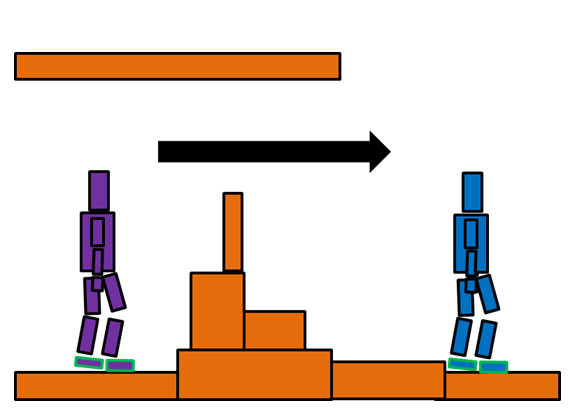
\includegraphics[width=0.25\textwidth]{Multicontact/MulticontactJustin/fig/rbprm1.png}} \quad
   \subfloat[Reachability planning]{ 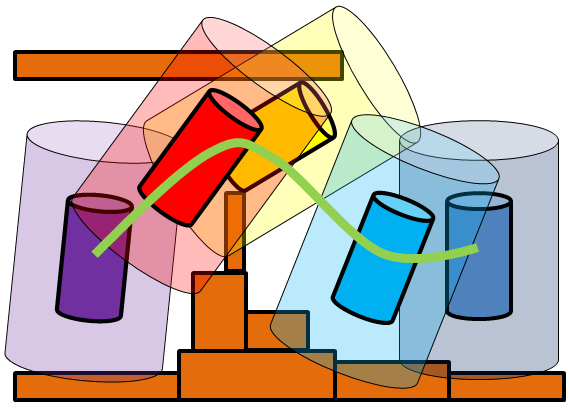
\includegraphics[width=0.25\textwidth]{Multicontact/MulticontactJustin/fig/rbprm2.png}} \quad
   \subfloat[Contact sequence]{ 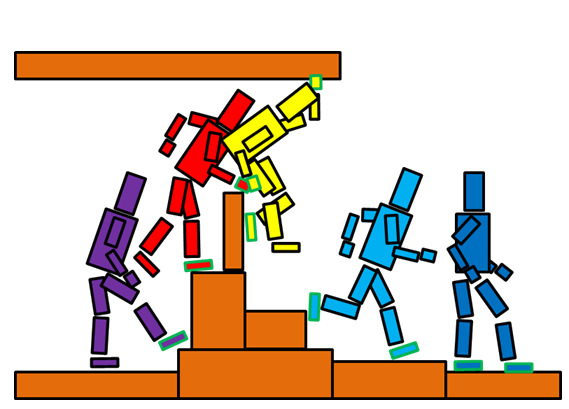
\includegraphics[width=0.25\textwidth]{Multicontact/MulticontactJustin/fig/rbprm3.png}}
    \caption{General principle of the contact planner. (a) The request is made by defining an initial and a final posture. (b) A central path is planned with the abstract shape, where the inside part of the shape should avoid collision while the outside part must stay in collision. (c) The central path is refined to compute a complete contact sequence.}
     \label{fig:rbprm}
   \end{center}
\end{figure*}

\subsection{The multiple shooting approach}

Problems \eqref{eq:ocpgen} and \eqref{eq:ocp} consider variables of infinite dimension and cannot be directly handled by a computer. Addressing these nominal problems requires the use of indirect results like Pontryagin's maximum principle or the dynamic programming, to reformulate the optimization problem as an integration problem of an augmented system. It is unlikely to solve \eqref{eq:ocp} this way due to the bilinear constraint~\eqref{eq:dyn_constraint2}. Alternatively, ``direct'' approaches turn the initial infinite-dimension problem into a finite-dimensional one by sampling the trajectory over an arbitrary function basis. 

Various details of implementation should be chosen to obtain an efficient resolution. The most important in our opinion is the way the pair $(\underline{\bm x},\underline{\bm u})$ is handled. 
Collocation \cite{qiu_dhm11,mordatch:tog:12} represents explicitly the state variable while the control is obtained from the state trajectory by inverting the system dynamics. On the other hand, single shooting \cite{tassa:icra:14,perrin_isrr15} represents explicitly the control trajectory while the state is obtained by integration. In between, multiple shooting represents explicitly the control trajectory along with some few state variables at given time instants. 

%Multiple shooting seems the most relevant solution for solving \eqref{eq:ocp}. First, t
Consider specifically the problem \eqref{eq:ocp}. The dynamics \eqref{eq:momentum} is numerically quite stable: collocation, which tends to be quite robust to unstable dynamics, is not necessary. On the other hand, it is relatively easy to build a good initial guess of the state trajectory, while a guess of the control trajectory is more complex to have: single shooting would be difficult to initialize, but both multiple-shooting and collocation are suitable. By elimination, multiple shooting is the best option.
%
We refer to \cite{FastMS} for more details on the aforementioned methods.
